\chapter{The Chandra Telescope and Analyzing X-ray Spectra Obtained with Chandra}
\section{Introduction to The Chandra X-ray Observatory}
The Chandra X-Ray Observatory (CXO) is a space observatory launched by NASA's Space Shuttle Columbia on July 23, 1999 with Col. Eileen Collins commanding. Chandra is the X-Ray component of NASA's four Great Observatories. The period of the Chandra is about 3809.3 minutes. The other three components are the Hubble Space Telescope, the late Compton Gamma-Ray Observatory and the Spitzer Space Telescope. Since the Earth's atmosphere absorbs the vast majority of X-rays coming from space, an X-ray telescope on the earth can not detect those X-rays. Therefore, space-based telescopes, like Chandra, are required to make the X-ray observations of astronomical objects. Chandra's spatial and spectral resolutions are order-of-magnitude better than previous X-ray telescopes \citep{ChandraMSFC}. Thanks to advances in technology, the Chandra telescope is sensitive to X-ray sources 100 times fainter than any other previous X-ray telescope.  \par

\subsection{Main Components of the Chandra Telescope}
Chandra consists of a spacecraft and a telescope/science-instrument payload. The observatory has four main components: The High Resolution Mirror Assembly (HRMA), the Aspect System, the Science Instruments (SIs) at the focal plane and the Transmission Gratings. See Fig.~\ref{fig:chandratelescope} for a diagram of the Chandra X-ray Observatory with main components labeled \citep{Harbaugh2017}. The SIs includes the Advanced CCD Imaging Spectrometer (ACIS) \citep{canizares2003} and the High Resolution Camera (HRC) . The Objective Transmission Gratings include High Energy Transmission Grating (HETG) \citep{Canizares2000} and Low Energy Transmission Grating (LETG) \citep{Brinkman2000} which together cover the energy range from $\leq 0.1$ to 10 keV.\par 

\begin{figure}[ht!]
\centering
  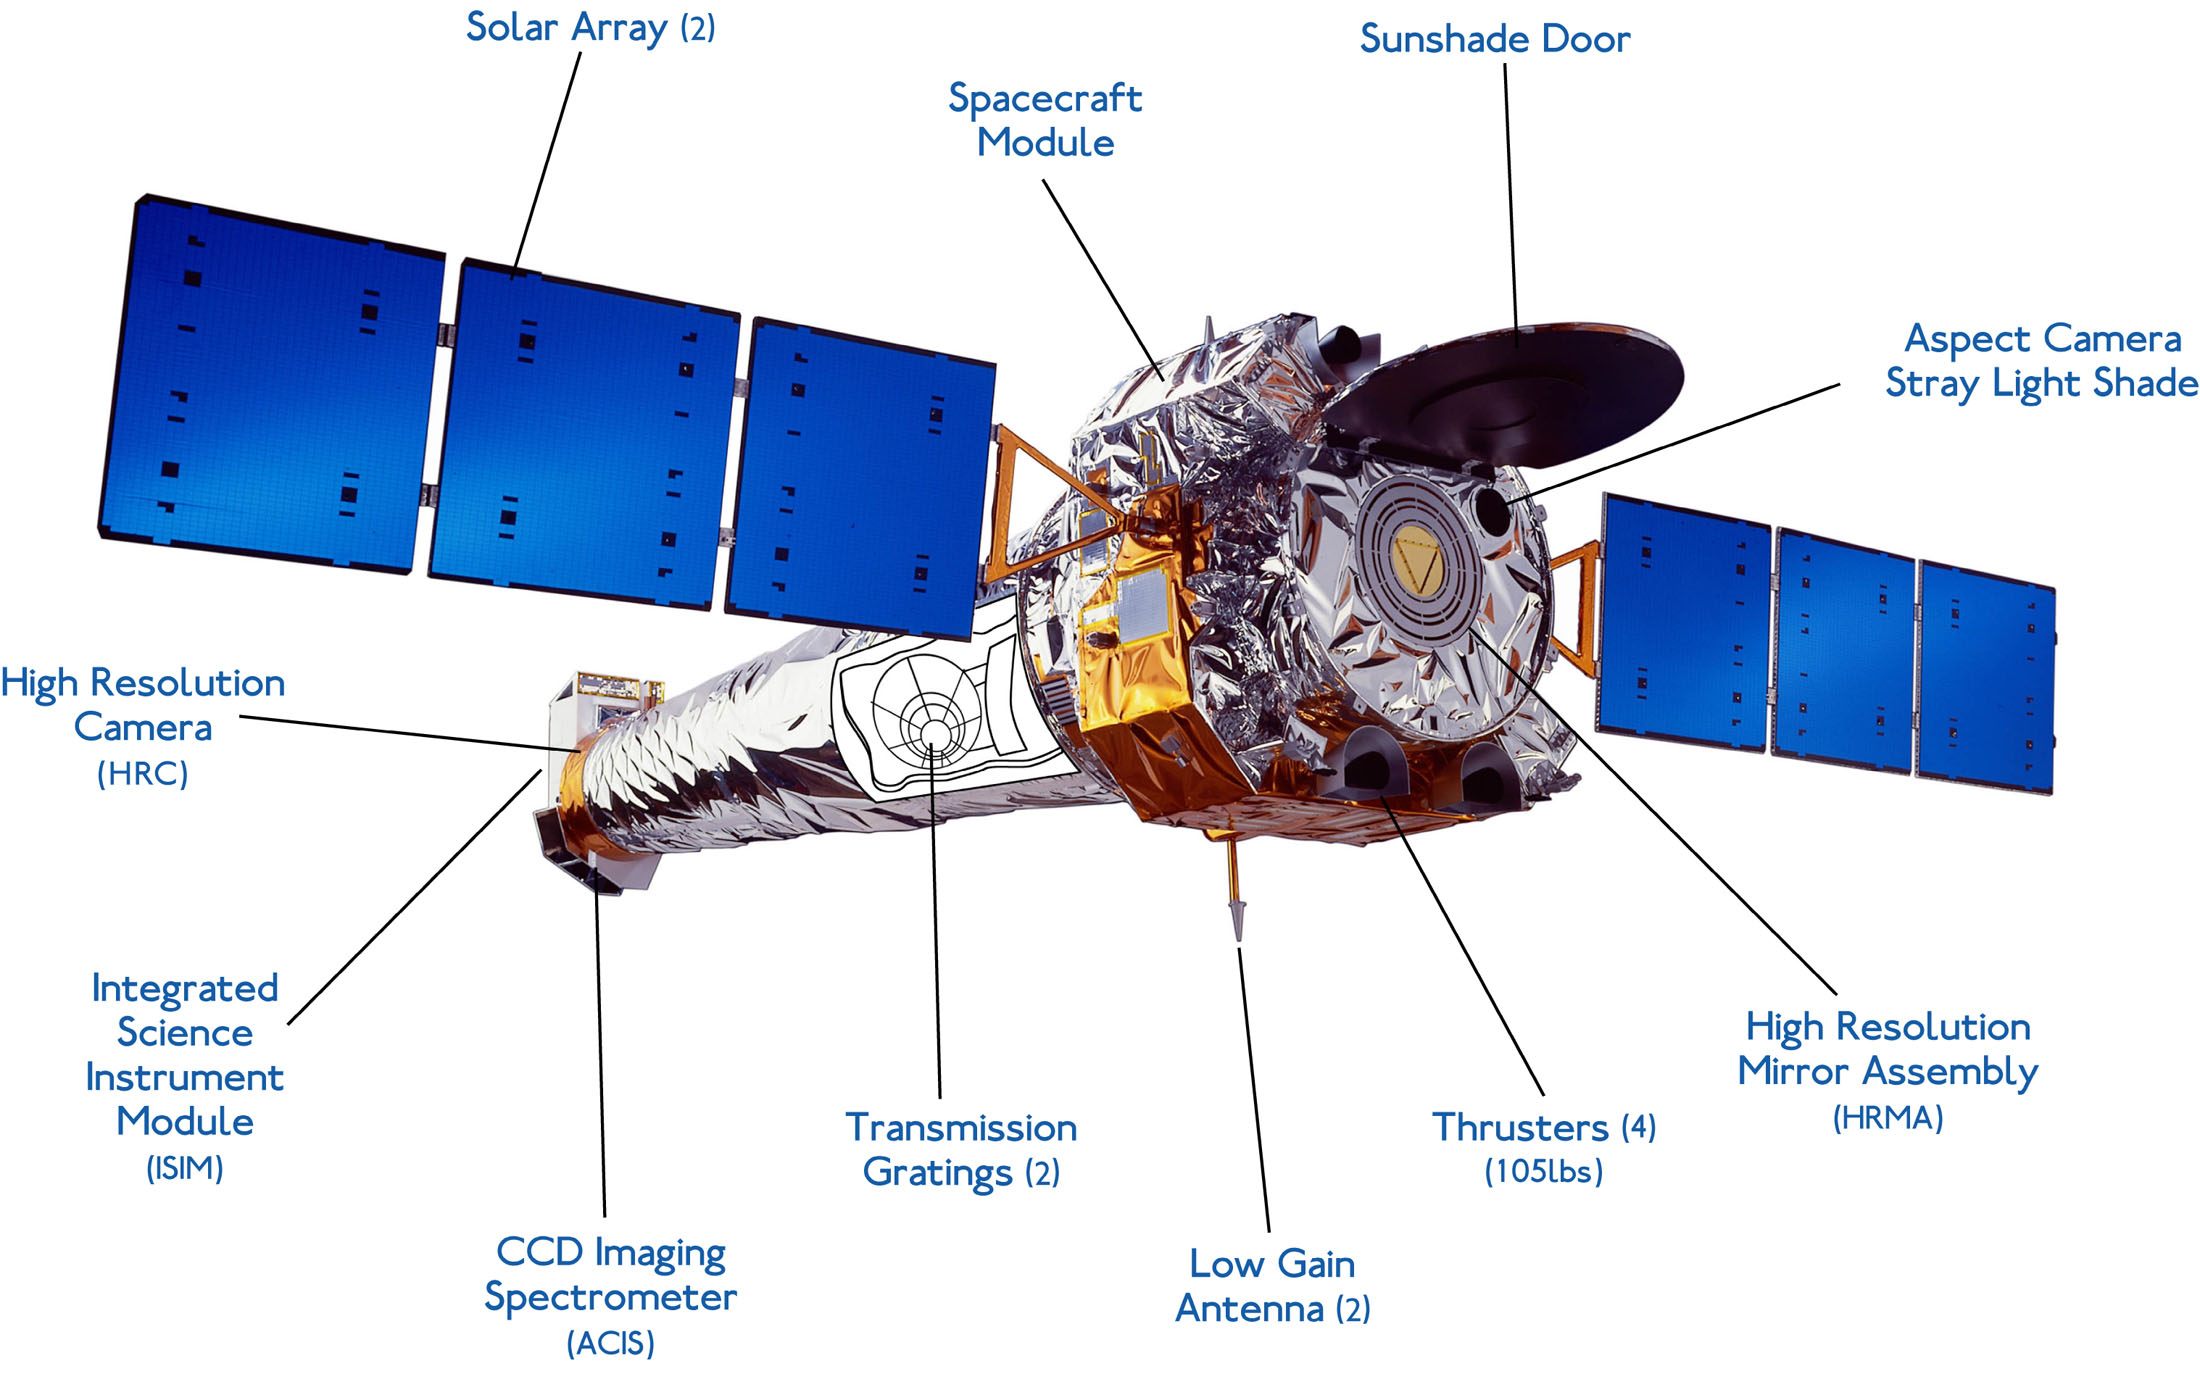
\includegraphics[width = \linewidth]{Chapters/Figures/chandra_full.jpg}
  \caption{The Chandra X-ray Observatory with main components labeled \citep{Harbaugh2017}}
  \label{fig:chandratelescope}
\end{figure}


\subsubsection{High Resolution Mirror Assembly (HRMA)}
The HRMA produces images with a half-power diameter of the point spread function of $<$ 0.5 arcsec. The HRMA consists of a nested set of four paraboloid-hyperboloid, grazing-incidence X-ray mirror pairs, with the largest having a diameter of 1.2 m. The effective focal length is 10 m. See Fig~\ref{fig:HRMA} for the sectional view of the HRMA of Chandra. X-rays that hit the mirror at grazing angles are reflected like a pebble skipping across a pond.\par

\begin{figure}[ht]
\centering
  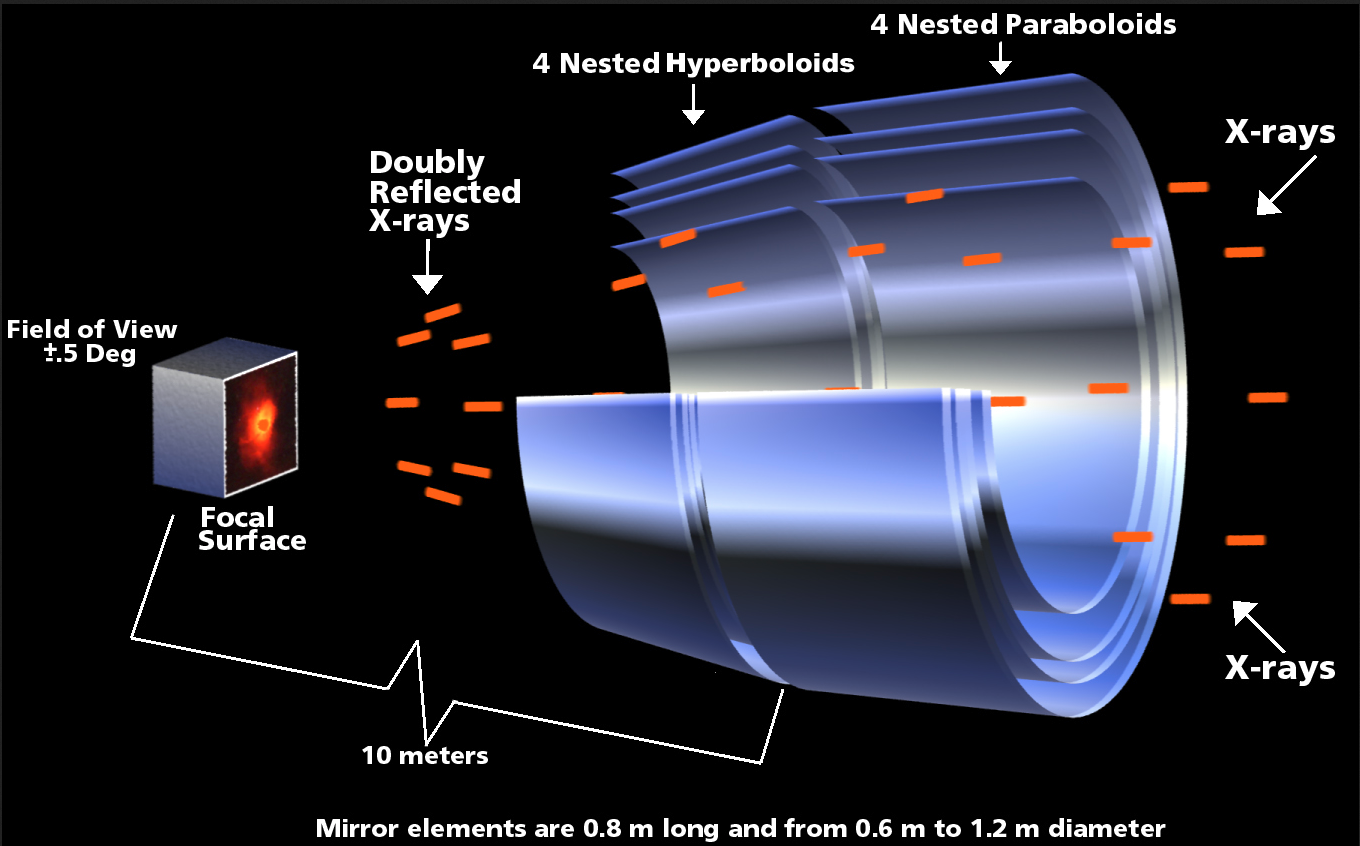
\includegraphics[width = \linewidth]{Chapters/Figures/paraboloid_hyperboloid_mirror.png}
  \caption{This cutaway illustrates the design and functioning of the High Resolution Mirror Assembly (HRMA) on Chandra \citep{NASA2009}.}
  \label{fig:HRMA}
\end{figure}


\subsubsection{The Science Instrument Module (SIM)}
The SIM contains the two detectors - the ACIS and the HRC. ACIS is composed of two CCD arrays, a 4-chip array, ACIS-I (16'$\times$16'), and a 6-chip array, ACIS-S (8'$\times$8') (See Figure \ref{fig:ACIS}).   


\begin{figure}[ht]
\centering
  \includegraphics[scale = 0.5]{Chapters/Figures/acis_def_chips_2.png}
  %\includegraphics[width=\linewidth]{acis_def_chips_2.png}
  \caption{A schematic drawing of the ACIS focal plane, not to scale \citep{ChandraMSFC}. ACIS-I and ACIS-S layout showing the imaging and spectroscopic arrays. The default aimpoints are marked with an x.}
  \label{fig:ACIS}
\end{figure}


\begin{figure}
    \centering
    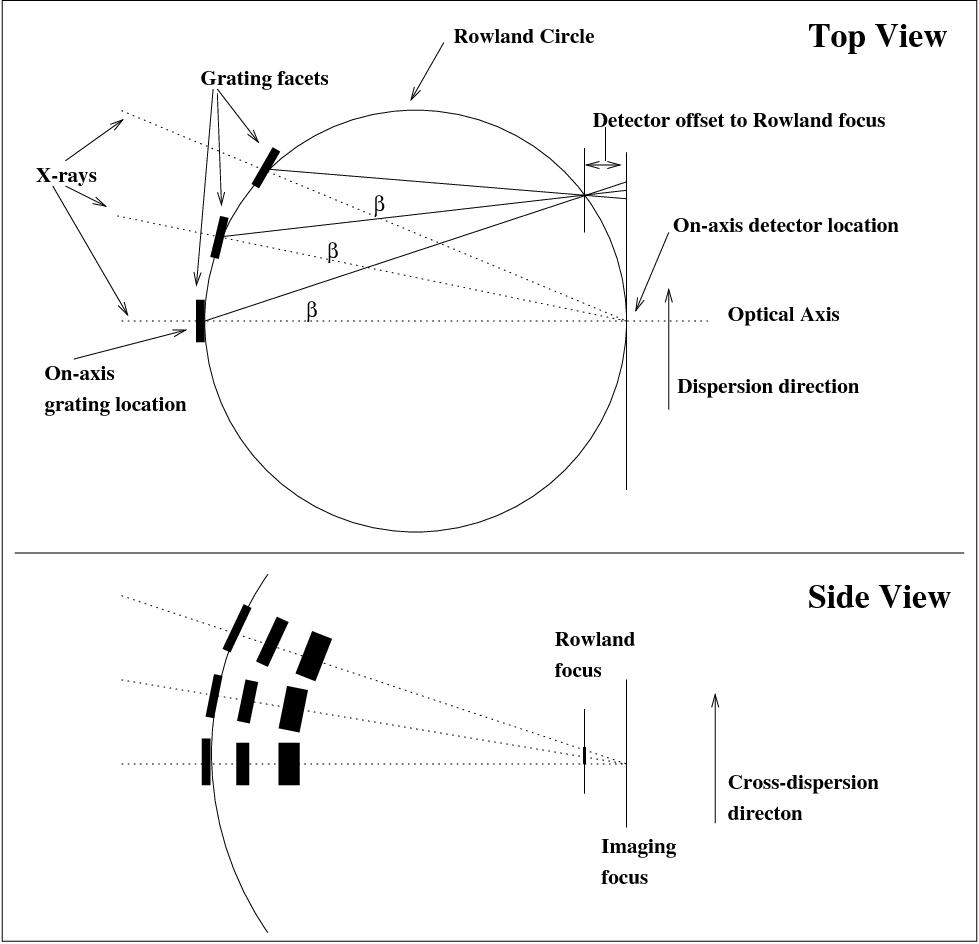
\includegraphics[width = 0.8 \linewidth]{Chapters/Figures/rowland.png}
    \caption{The Rowland geometry is shown schematically. In the ``Top'' view, the diffraction angle is $\beta$. The geometry is such that converging rays are diffracted at a specific angle by the gratings (which are located on the Rowland circle). Then the rays converge to a point that is also on the Rowland circle. The dotted lines show zeroth-order rays, which will be focused at the middle point of the other side of the Rowland circle. The solid lines represent the grating-diffracted first-order rays. The bottom panel (``Side'' view) looks along the dispersion direction at rays from a set of gratings arranged perpendicularly to those in the ``Top'' view. Since the converging rays have not yet reached the imaging focus, the spectra are extended perpendicular to the dispersion direction by less than 100 microns \citep{ChandraMSFC}.}
    \label{rowland}
\end{figure}


ACIS-I is usually better for direct imaging, and the ACIS-S is better suited for spectroscopy with the High-Energy Transmission Grating system. The CCDs detect X-ray photons individually and records their position on the detector, energy and arrival time. \par 



\subsubsection{The High Energy Transmission Grating (HETG)}

The HETG works with the High Resolution Mirror Assembly (HRMA) and a focal-plane imager for high resolution spectroscopy. The complete instrument is called the High-Energy Transmission Grating Spectrometer (HETGS). The HETGS achieves high resolution spectra (with $E/\Delta E$ up to 1000) between 0.4 keV and 10.0 keV energy range \citep{ChandraMSFC}. Standard processing of an HETG system observation produces spectrometer information products: PHA (Pulse Height Amplitude, the raw spectrum), ARF (Ancillary Response File) and RMF (Response Matrix File), the instrument calibration files). The HETG consists of two sets of grating assemblies - the High Energy Grating (HEG) and the Medium Energy Grating (MEG). The HEG diffracts X-rays from only the two inner mirror shells and the MEG diffracts X-rays from only the two outer mirror shells. \par
The HETGS-faceted Rowland design is shown in Figure~\ref{rowland}. The Rowland geometry of the grating plate and spectroscopic arrays minimize dispersed image aberrations so as to maintain the telescope's focal properties in the dispersion direction. As a result, Rowland geometry contributes to improved spectral resolution \citep{ChandraMSFC}. 


\begin{figure}[ht!]
\centering
  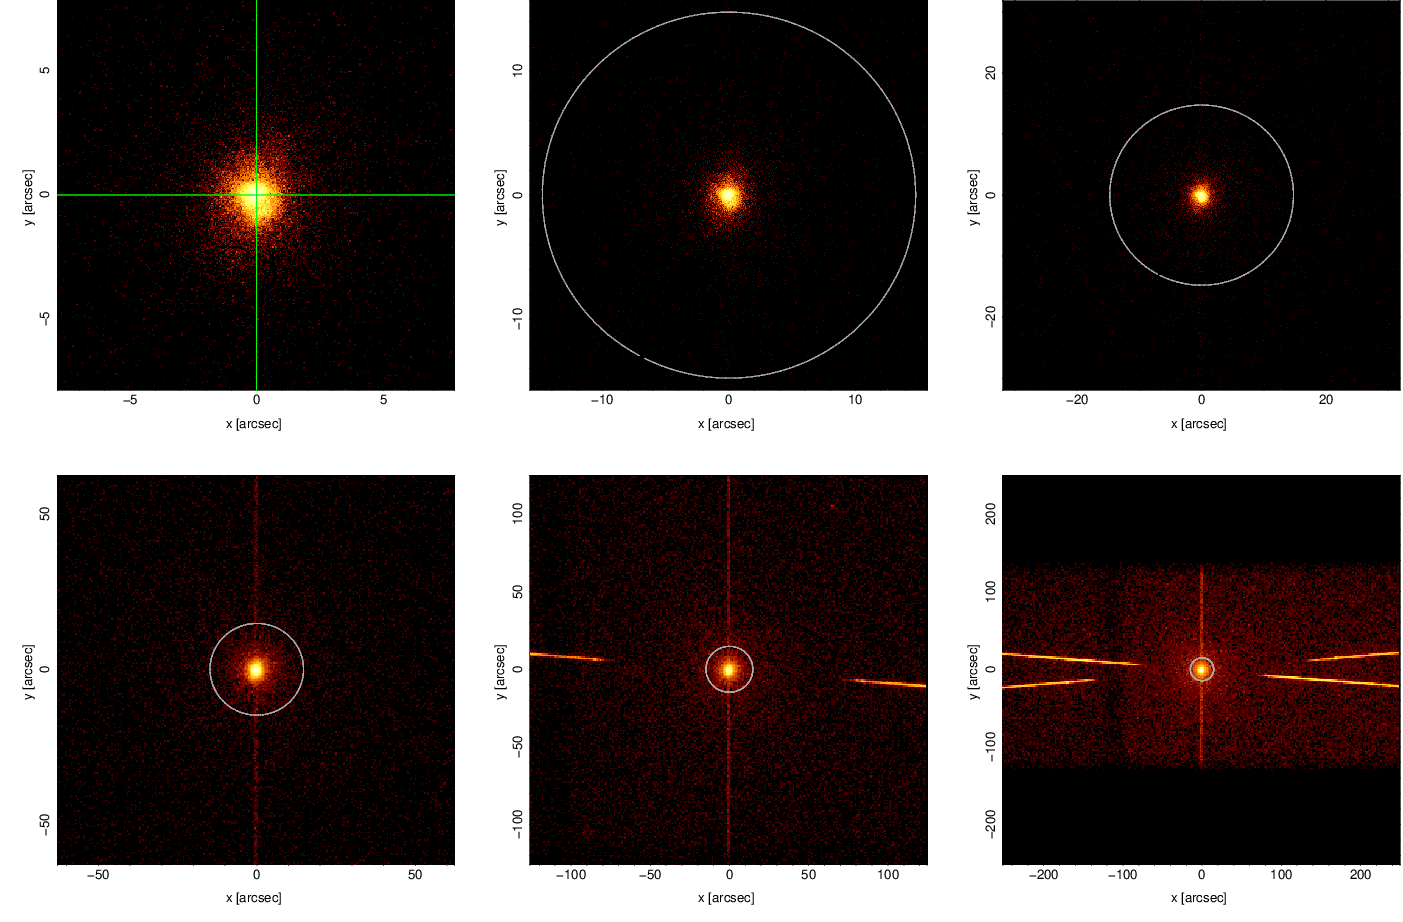
\includegraphics[scale=.3]{Chapters/Figures/X_orders.png}
  \caption{The top panel shows the bright zeroth order. The bottom panel shows the HETGS diffracted X pattern, yielding the first-order spectrum. }
  \label{xpattern}
\end{figure}

Figure~\ref{skyfield} shows the MEG and HEG spectra forming an ``X'' pattern. The bright zeroth-order image is visible at the aim point. The opening angle between the MEG and HEG is 9.96$\degree$. The first order (minus and plus) is followed by the zeroth order along the arms and so on. The spectroscopic array spans approximately $8'\times 48'$ of the sky. Wavelengths are assigned depending on how far the events are from the zeroth-order image. If X-rays of wavelength $\lambda$ hit the transmissions gratings and are diffracted (in one dimension) by the dispersion angle $\beta$, then according to the grating equation, we have
\begin{equation}
    sin\beta = m\lambda/p
\end{equation}
where $m$ is the integer order number and $p$ is the spatial period of the grating lines.
The HEG range is 15 - 1.2 \AA (0.83 -10.0 keV). The MEG range is 31 - 2.5 \AA (0.4 - 5 keV).\par

The HETG support structure (HESS) is a circular aluminum plate that is 110 cm in diameter and 6.35 cm thick \citep{ChandraMSFC}. HESS swings on and off depending on whether the images needed to be dispersed or not. There are 336 grating facets mounted on the HESS, each about 25 mm square \citep{ChandraMSFC}. Figure~\ref{hess} shows front and side view of the HESS. The two outer annuli have 192 MEG gratings and the two inner annuli have 144 HEG gratings. Every grating within one ring is mounted in the same direction such that X-rays coming to the gratings on the same ring will diffract at the same angle. The two sets of gratings are mounted with at different angles so that the dispersed images from the HEG and MEG will form a shallow X centered at the undispersed (zeroth order) position. A detailed schematic layout of HETGS is shown in Figure~\ref{hetgs}.\par 


\begin{figure}
    \centering
    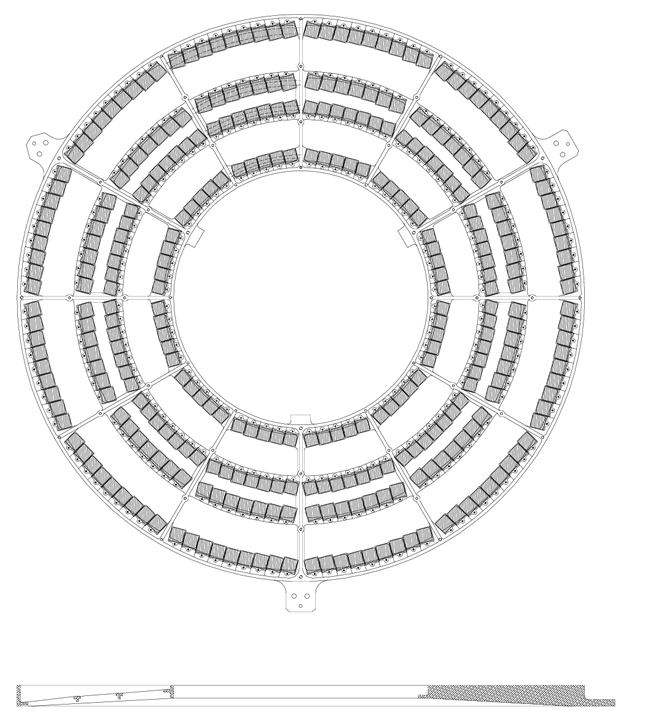
\includegraphics[width = 0.5\linewidth]{Chapters/Figures/hess.png}
    \caption{The upper and the lower figures show the front and the side view of the HESS, respectively. The front view is seen from the view of X-rays; the X-ray intercept with the grating facets as they leave the HRMA. In the side view, the left part shows the four support rings that are in different planes due to the Rowland curvature \citep{ChandraMSFC}.}
    \label{hess}
\end{figure}

\begin{figure}
    \centering
    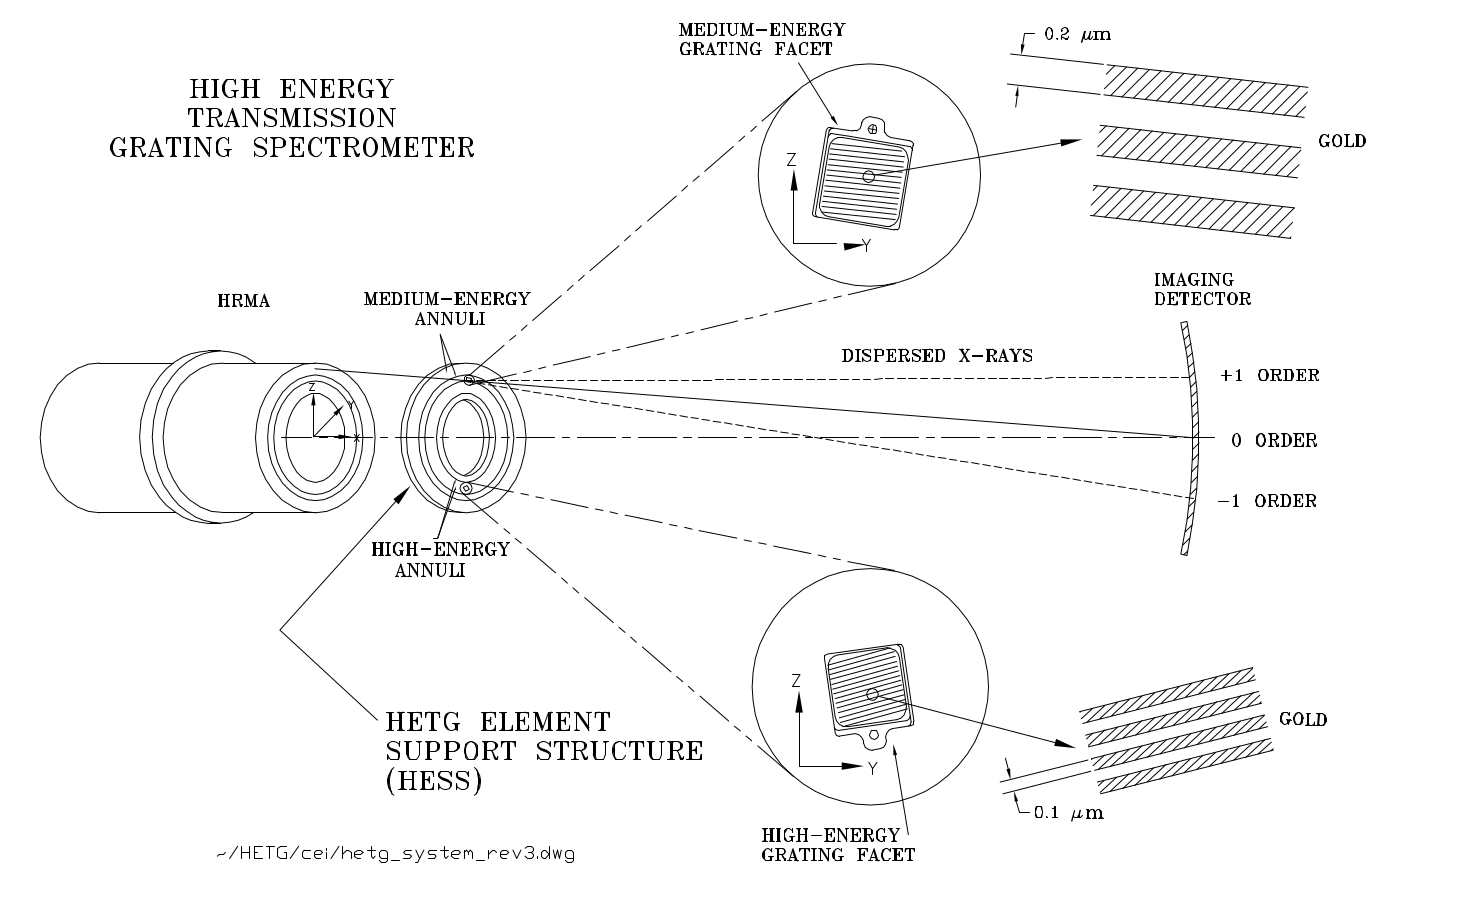
\includegraphics[width = 0.6\linewidth]{Chapters/Figures/hetgs.png}
    \caption{A schematic layout of the High Energy Transmission Grating Spectrometer \citep{ChandraMSFC}.}
    \label{hetgs}
\end{figure}

The HETG grating facets are made of electro-plated gold bars supported on a polyimide substrate. Figure~\ref{facet} shows a life-size model of the HESS with a few grating facets on it. This unit is currently in Dr. Herman Marshall's lab in MIT Kavli Institute.



\begin{figure}
    \centering
    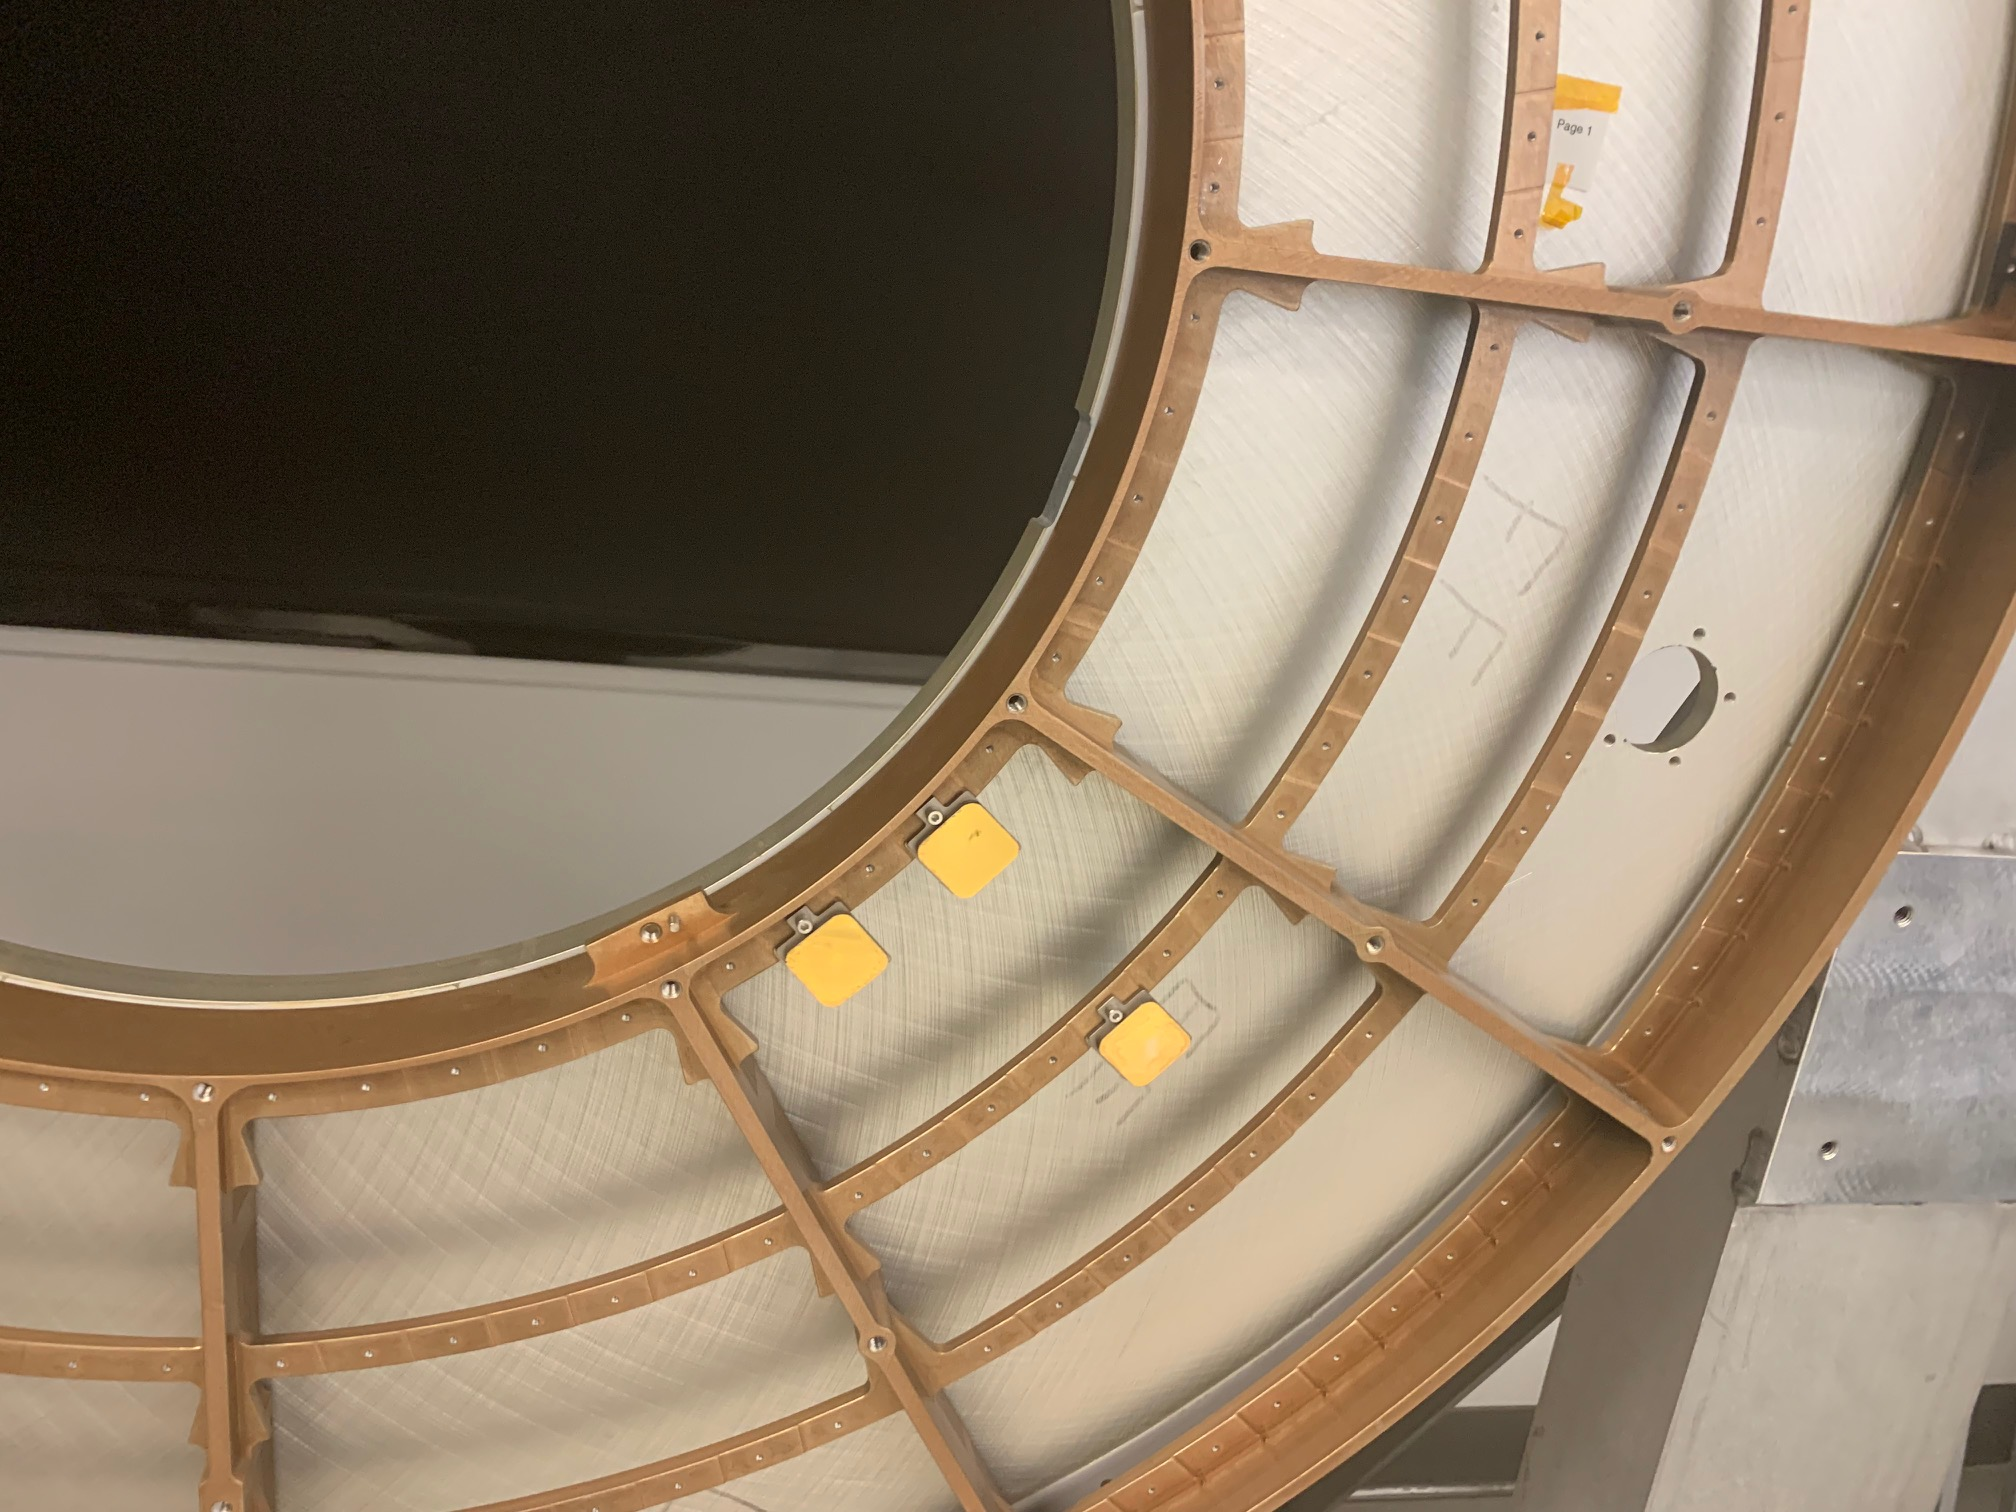
\includegraphics[width = 0.6\linewidth]{Chapters/Figures/facet.jpg}
    \caption{A portion of a life-size model of the HESS at MIT/CXC showing three HEG grating facets and the support frames (image taken by the author of this thesis).}
    \label{facet}
\end{figure}




\section{High resolution X-ray spectral Analysis}
\subsection{Data Preparation}

\subsubsection{Detecting X-rays with Chandra}
The ACIS detector consists of CCDs chips that can record not only the positions of the photons on the detector, but also the photon's energy and time of arrival. However, there are instrumental issues that affect how photons of a given energy are redistributed into a number of ACIS detector channels. The formal description of the transformation from photons to counts is
\begin{equation}
    C(h) = T\int_0^{\infty}\sum_i R_i (E, h)A_i(E)S_i(E)dE + B(h),
\end{equation}

where 
\begin{itemize}
    \item $C(h)$ is the number of counts in detector channel $h$, \item $T$ is the exposure time,
    \item $R_i(E,h)$ is the detector redistribution from energy E to channel $h$ (This information is encoded in Response Matrix File, or RMF, that is generated for every observation) for the source component $i$,
    \item  $A_i(E)$ is the effective area (geometric area $\times$ filter efficiency $\times$ detector quantum efficiency)(This information is encoded in Ancillary Response File, or ARF, that is also generated for every observation) at energy E for source component $i$,
    \item $S_i(E)$ is the source photon flux at energy E for component $i$,
    \item $B(h)$ is the background counts in channel $h$. This could include both cosmic and internal sources, empirical or modeled, possibly from other observations \citep{Huenemoerder_lec_2011}.
\end{itemize} 

The basic data product from which all analysis follows is the \textit{event list} provided as a Flexible Image Transport System (FITS) binary table, which includes information such as time, detector element ID, detector X pixel, detector Y pixel, pulse height amplitude (PHA), etc \citep{Huenemoerder_lec_2011}.\par


% An HETGS count spectrum produced by standard analysis (a PHA file) can be related to the source spectrum through a grating ARF (Auxiliary Response File) and grating RMF (Redistribution Matrix File).\par 

The ARF contains the effective area as a function of energy for an observation \citep{Huenemoerder_lec_2011}. When a physical spectrum is multiplied by an ARF, the result would be the distribution of counts that received by a detector. The ARF includes the efficiencies of mirrors, gratings, filters and detector.  Figure~\ref{effective} shows an example of effective area vs. energy graph. Edges in the graph are due to different non-uniformities.


\begin{figure}[ht!]
\centering
  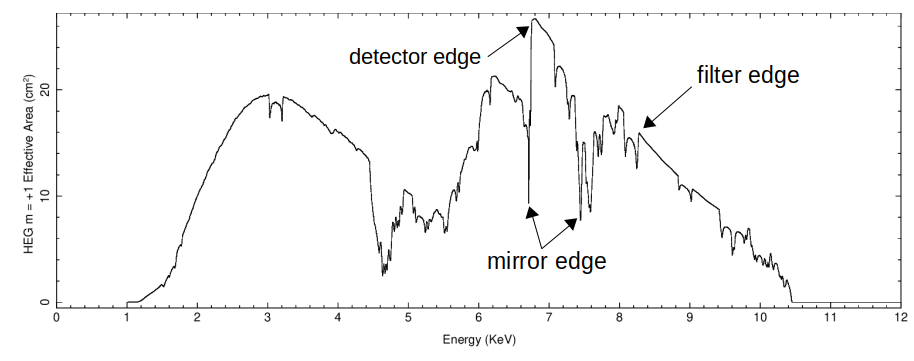
\includegraphics[width = \linewidth]{Chapters/Figures/effective_area_label.png}
  \caption{The HETGS HEG +1 effective area from an ARF file of 2018 Chandra observation. Edges of detector, mirror and filter are labeled in the graph.}
  \label{effective}
\end{figure}


An RMF is a standardized format FITS file that encodes the relationship between the incident photon energy and the output signal's distribution over channels (such as detector pulse heights or PHA).  High energy photons encounter detector and interact with the detector material (e.g., silicon for CCDs). When a photon is absorbed in the silicon of a CCD, a charge cloud of electron-hole pairs is formed ($\approx$ 3.65 eV per pair)\citep{Davis2008}. PHA is a measure of the number of pairs in the cloud. The response matrix accounts for how the
detector redistributes photons of a given
energy. Figure~\ref{rmf} shows the visualization of the RMF of the ACIS-S3 chip. For photons of energy E, there is a probability distribution that describes how many counts can be expected in each detector channel. As incoming photon energy increases, the peak of the distribution shifts to greater
pulse height amplitudes, or detector
channel. When modeling a Chandra X-ray spectrum, the source model must first be multiplied by the effective area curve. Then the result is multiplied by the response matrix that redistributes modeled photon flux into detector channels. The final result is a model X-ray spectrum of counts vs. pulse height amplitude, which can be compared to the observed X-ray spectrum \citep{Doe2009}.

\begin{figure}[ht!]
    \centering
    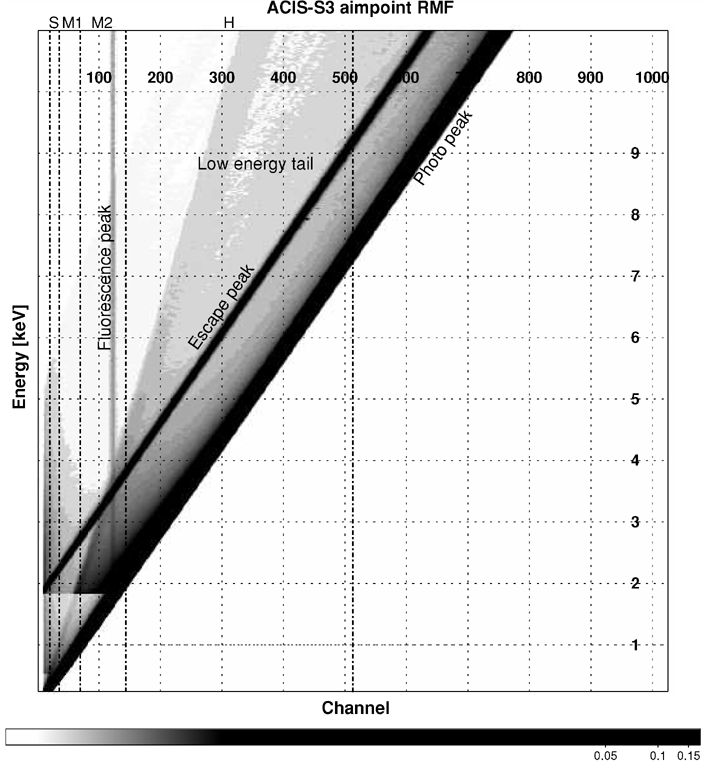
\includegraphics[width = 0.7\linewidth]{Chapters/Figures/rmf.png}
    \caption{Response matrices ACIS-S3 at the aim point. Grayscale is logarithmic. Numbers on the right-hand side are energy in units of keV and numbers at the top are PHA/PI channel numbers. The vertical dash-dotted lines delimit the energy bands \citep{Grimm2009}.}
    \label{rmf}
\end{figure}


\subsubsection{Software and Data Analysis}

Prior to starting HETG data analysis, few software packages need to be downloaded and installed. ISIS \citep{Houck2000} denotes the Interactive Spectral Interpretation System, which supports the analysis of high resolution X-ray spectra using the database of atomic data and plasma emission models. CIAO tool \citep{CIAO2006} is the software package developed by the Chandra X-Ray Center for analyzing data from the Chandra X-ray Telescope. TGCAT denotes The Chandra Transmission Gratings Archive and Catalog, which makes grating spectra easily viewable and analyzable \citep{Huenemoerder2011}. Data processing for the TGCAT catalog is done with a collection of ISIS/S-Lang scripts. TGCAT uses both CIAO and ISIS\par

The first step is to download observations from the online Chandra data archive and configure the data directories to optimize our processing requirements. Then we set the ISIS and CIAO environment so that necessary tools are in the path. We then use TGCAT to extract the PHA, ARF, RMF, as well as the summary plots. The detailed files generated are as follows. 
\begin{itemize}
    \item \textbf{evt0.par} An ASCII file listing header keywords and values from the event file.
    \item \textbf{evt1} The level 1 event file that contains all the events recorded for the observation.
    \item \textbf{evt2} The level 2 event file created by the level 1 event file. A FITS binary table, containing the grating coordinates, time, and other information for each good event. 
    \item \textbf{\*\_\#.arf} ``Ancillary Response Files'' for different gratings. \# is a diffraction order, either -1 or 1. 
    \item \textbf{\*\_\#.rmf} ``Response Matrix Files'' for different gratings. \# is a diffraction order, either -1 or 1. 
    \item \textbf{pha2\*} ``Pulse Height Amplitude'' files for binned spectrum and binned background
    \item \textbf{summary\_flux\_overview.ps} Overview flux spectrum plot
    \item \textbf{summary\_fprops.fits} Flux properties (FITS binary table). Contains counts and rates summed in bands. For coarse characterization. 
    \item \textbf{summary\_[hm]eg}  Order sorting image (FITS image), for all photons.
    \item \textbf{summary\_[hm]eg\_all.fits (H)} Order sorting image (FITS image), for filtered, binned photons. 
    \item \textbf{summary\_im-a.ps} Summary image; source region detail (Figure~\ref{xpattern})
    \item \textbf{summary\_im-b.ps} Summary image; sky field image (Figure~\ref{skyfield}).
    \item \textbf{summary\_imsp.ps} Summary image; spectral-spatial image 
    \item \textbf{summary\_lc.ps } Summary plot; light curve 
    \item \textbf{summary\_spc.ps } Summary plot; counts (Figure~\ref{spc})
    \item \textbf{summary\_spf.ps} Summary plot; flux (Figure~\ref{spf})
\end{itemize}

\begin{figure}[ht!]
    \centering
    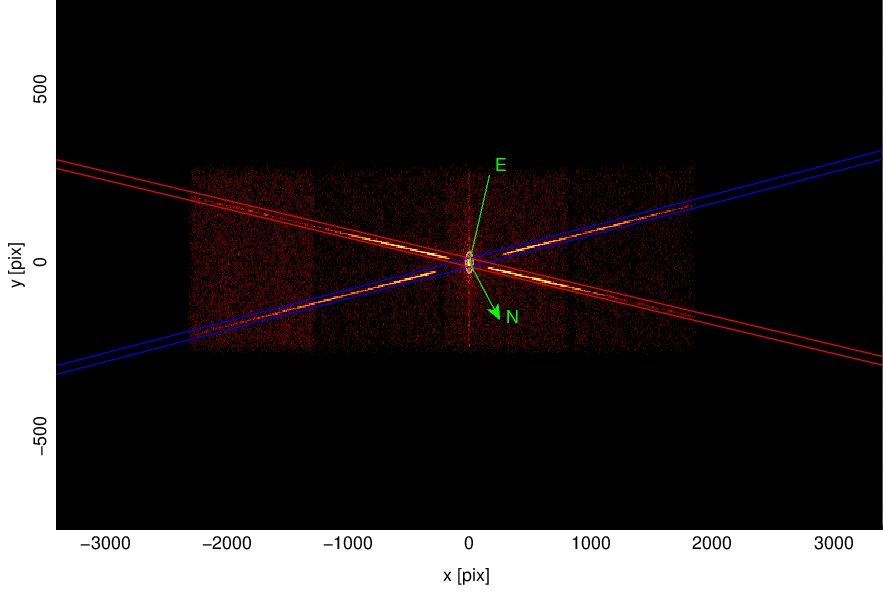
\includegraphics[width = \linewidth]{Chapters/Figures/sky_field.png}
    \caption{An ``X'' pattern of the spectrum. The blue line shows the high energy spectrum and the red line shows the medium energy spectrum.}
    \label{skyfield}
\end{figure}

\begin{figure}[ht!]
    \begin{minipage}[t]{0.45\textwidth}
        \centering
        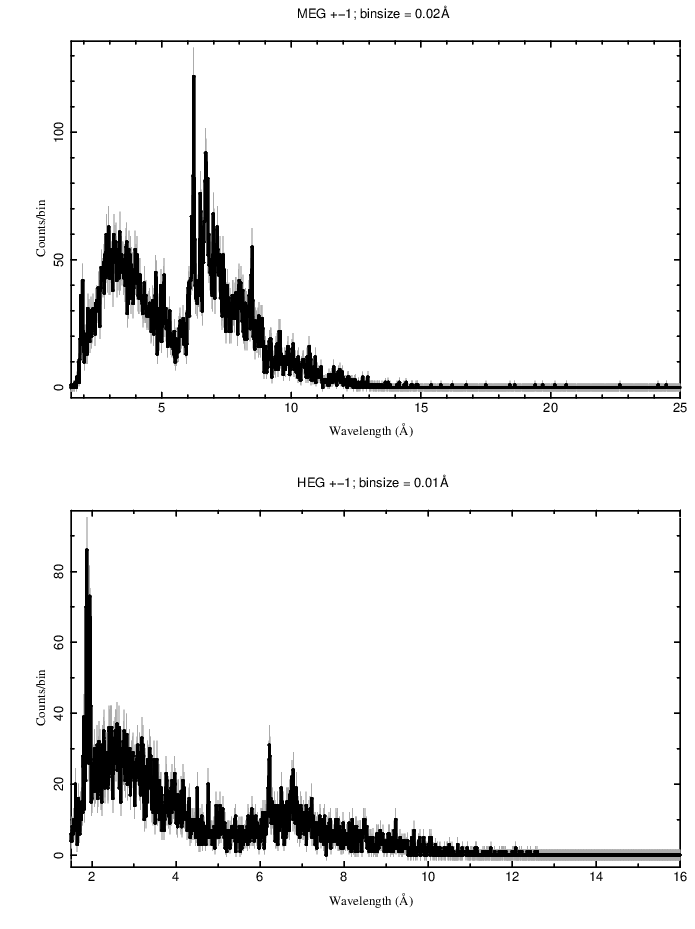
\includegraphics[scale = 0.3]{Chapters/Figures/spc.png}
        \caption{Counts vs. wavelength spectral plot.}
        \label{spc}
    \end{minipage}
    \begin{minipage}[t]{0.6\textwidth}
        \centering
        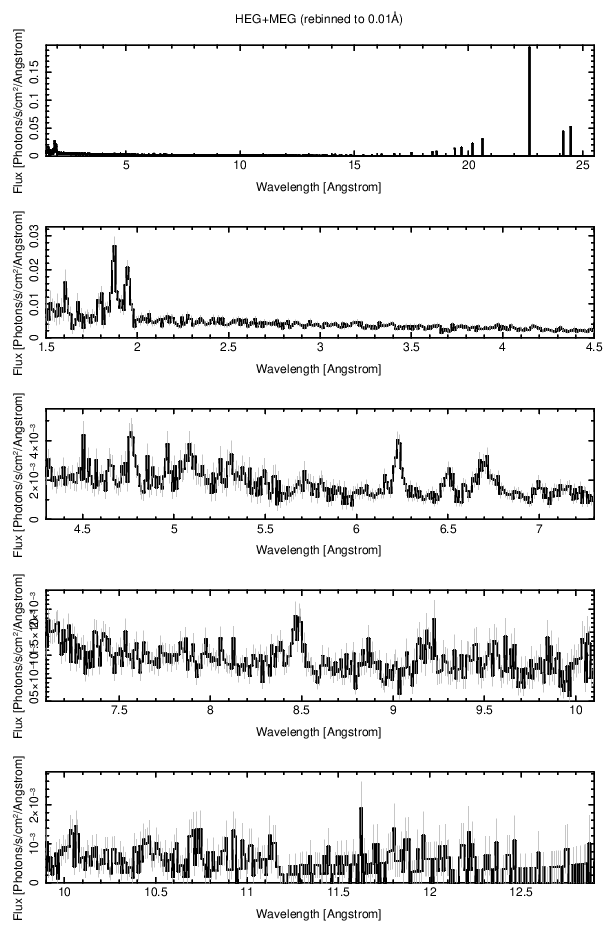
\includegraphics[scale = 0.35]{Chapters/Figures/spf.png}
        \caption{Flux vs. wavelength spectral plot.}
        \label{spf}
    \end{minipage}
\end{figure}




\subsection{Choosing the Right Fit Statistic}
Parameter estimation performed in ISIS finds the parameters for a given model that fit the data best. Statistics estimates the uncertainties on these parameters and tests whether model's best-fit parameters match with the data. \citep{Arnaud1999}. \par 
Which statistics to use depends on the probability distributions underlying the data. Almost all astronomical data are drawn from one of two distributions: Gaussian or Poisson \citep{Arnaud1999}. Poisson distribution is valid if the only source of the experimental noise is due to the number of events arriving at the detector, for example, modern CCD instruments \citep{Arnaud1999}. If some other sorts of noise is significant then it could be described by the Gaussian distribution. One common example would be background needs to be modeled in some way, rather than directly measured. The uncertainty in the background modelling is assumed to be Gaussian \citep{Arnaud1999}. \par

In order to assess the validity of models, hypothesis test can be formulated about astrophysical process. A well-known test is based on Pearson’s $\chi^2$ statistic
\begin{equation}
    S \equiv \sum_{i = 1}^{N}\dfrac{(D_i - F_i)^2}{\sigma^2}
    \label{chi}
\end{equation}
where $D_i$ is the number of observed counts in bin $i$, $F_i$ are the number of counts predicted by the model and $\sigma_i^2 = F_i$ is the deviations which are approximately Gaussian \citep{Lampton1976}. 

It is easier to obtain the best-fit parameters of the model by minimizing $\chi^2$ when $\sigma_i^2$ is approximated by a large source intensity. However, X-ray spectra of astrophysical sources are often characterized by relatively low amounts of counts per spectral bin.  Chi-squared test doesn't work well when there are low numbers of counts per spectral bin \citep{Kaastra2017}. From Equation~\ref{chi}, we can see that it fails for small source intensity by putting $\sigma_i$ = 0 in the equation.\par 
Another method found by Webster Cash solved this problem \citep{Cash1979}. The discrete Poisson distribution:
\begin{equation}
    \text{prob}(D_i) = p(D_i|M_i) = \dfrac{M_i^{D_i}}{D_i!}e^{-M_i}
    \label{poisson}
\end{equation}
which represents the probability of finding $D_i$ event (counts) in bin $i$ (energy range) of data set D (spectrum) in a given length of time (exposure time), if the events occur independently at a constant rate $M_i$ (source intensity) \citep{Siemiginowska09}.\par 

In order to find the best parameter $M_i$ to fit the model the data better, it is natural to maximize the product of Poisson probabilities in each data bin $i$, i.e., to maximize the Poisson likelihood.

\begin{equation}
    L = \prod_i^{N} \dfrac{M_i^{D_i}}{D_i!}e^{-M_i} =\prod_i^{N} p(D_i|M_i)
    \label{maxhood}
\end{equation}

In practice, what is often maximized is the -2 log-likelyhood. After taking -2log of Equation~\ref{maxhood}, it becomes 
\begin{equation}
    C = 2\sum_i^{N} (M_i - D_i\mathrm{log}M_i) \propto -2L
    \label{cash}
\end{equation}
This is a well known statistic in X-ray astronomy which is called ``Cash Statistic''.\par 
 
 
 
 
 
 
 
 
 
 
 
 
 
 
 
 
 
 
 
%  The goodness of fit is expressed as 
% \begin{equation}
%     \chi^2 = \displaystyle\sum_{i=1}^n \dfrac{(M_i - s_i)^2}{\sigma_i^2}
%     \label{chisq}
% \end{equation}
% where the summation over i is over all n bins of the spectrum, $M_i$ is the observed number of counts, $s_i$ is the expected number of counts for the tested model, and $\sigma_i^2 = s_i$ for Poissonian statistics \citep{} \par 

%  Also, considering the data in a bin is downward fluctuation. Since we estimate the variance (in the denominator) using the observed data, the downward fluctuation contributes more to chi-squared than an upward fluctuation, resulting the biased best-fit model \citep{arnaud2012}. Therefore, it is not a proper method for spectrum that has small amount of counts per bin. Although there are methods to improve this problem, drawbacks still exist. For example, \cite{Gehrels1986} approximation for $M_i$ causes problems when the spectra are rebinned \citep{Kaastra2017}. \par 
% It was found out by \cite{Cash1979} that 
% \begin{equation}
%     \Tilde{C} = 2\displaystyle\sum_{i = 1}^n s_i - M_i\ln{(s_i)}
%     \label{cash}
% \end{equation}
% is a better statistics and can be applied to bins with a small number of counts. In Equation~\ref{cash}, $M_i$ is not in the denominator, so we do not need to worry about problems caused by upward or downward fluctuations.\par 






 








%\end{document}